\label{chap:discussion}

This chapter synthesizes the quantitative findings from the DSPI and the qualitative insights from the automated classifcation pipeline to answer the research questions. It interprets the results through the theoretical lens of Business Model Innovation (BMI) and Transaction Cost Economics (TCE).

\section{The Strategic Archetypes of Geo-Arbitrage}
Based on the analysis of Terms of Service and corporate enforcement actions across our expanded sample ($N=11$), we identify three distinct strategic archetypes that govern how digital firms respond to price arbitrage:

\subsection{The Content Fortress (Coercive)}
Firms adhering to this strategy, typified by streaming giants like \textbf{Netflix} and \textbf{Disney+}, prioritize the maintenance of regional licensing agreements over user convenience. Our quantitative analysis reveals that within the "Content Licensing Sector," the specific correlation between price variance and enforcement is negligible ($R \approx 0.006$). This indicates that strict enforcement is not a *reaction* to specific price arbitrage risks, but an \textbf{industry standard}—a baseline requirement for operating a licensed streaming service. \textbf{Disney+} and \textbf{Netflix} allocate approximately \textbf{8.5\%} and \textbf{6.2\%} of their enforcement clauses to \textbf{Content Licensing} issues, respectively.

This aligns with the "Fortress" strategy described by \textcite{schmidt2020transnational}, where incumbent firms build digital walls to protect legacy revenue streams. However, as noted by \textcite{lobato2019geoblocking}, such strategies often suffer from a "legibility" problem—users do not see the legal contracts, only the "This content is not available" error.

\subsection{The Ecosystem Fortress (Adaptive)}
In contrast, platforms like \textbf{Apple Music} exemplify a "Globalist" or adaptive approach. With negligible focus on \textbf{Technical Blocking} (0.15\%) and a strong emphasis on \textbf{Price Discrimination} (5.7\%), Apple appears to accept the reality of the international "ibusiness" fragmentation described by \textcite{brouthers2016explaining}. Rather than fighting a futile technological war against security compromises \parencite{ransbotham2009choice}, they focus on minimizing transaction costs through hardware and payment integration.

\subsection{The Enterprise Fortress (Defensive)}
A new archetype identified in this study is the "Enterprise Fortress," exemplified by \textbf{Microsoft}. Despite having the lowest global price variance in the dataset (indicating a relatively harmonized global price for Microsoft 365), Microsoft exhibits the highest intensity of "Account Action" clauses. This suggests that for utility software, enforcement is not driven by *geo-arbitrage* (pennies on the dollar) but by *license compliance* and *security*. The "Fortress" is built to keep unauthorized resellers out, not necessarily to stop a user from saving \$2 a month.

\subsection{The Utility Paradox (Adobe)}
\textbf{Adobe} presents a unique case. It has high price discrimination (similar to Netflix) but relatively low "Technical Blocking" enforcement. This is likely because Adobe's enforcement mechanism is "on-device" (software activation keys) rather than "on-network" (IP filtering). This highlights that "Technical Blocking" is a strategy specific to *cloud-streamed* content, whereas *downloaded software* relies on different protection mechanisms.

However, a hybrid future is emerging in the form of \textbf{"Always-Online DRM"}. Features like Adobe's "Generative Fill" require strictly authenticated cloud connections to function, effectively merging the "Content Fortress" reliance on IP checks with the "Enterprise Fortress" reliance on strong identity. This reflects the "Opportunities and Risks" of SaaS adoption \parencite{benlian2011opportunities}, where the control shifts completely from the client to the cloud provider, rendering traditional offline circumvention obsolete.
\subsection{The Cat-and-Mouse Game: A Longitudinal View}
The adversarial relationship between providers and consumers is not static. Our historical analysis reveals a clear "Action-Reaction" cycle, which we visualize in Figure \ref{fig:timeline}.

\begin{figure}[ht]
    \centering
    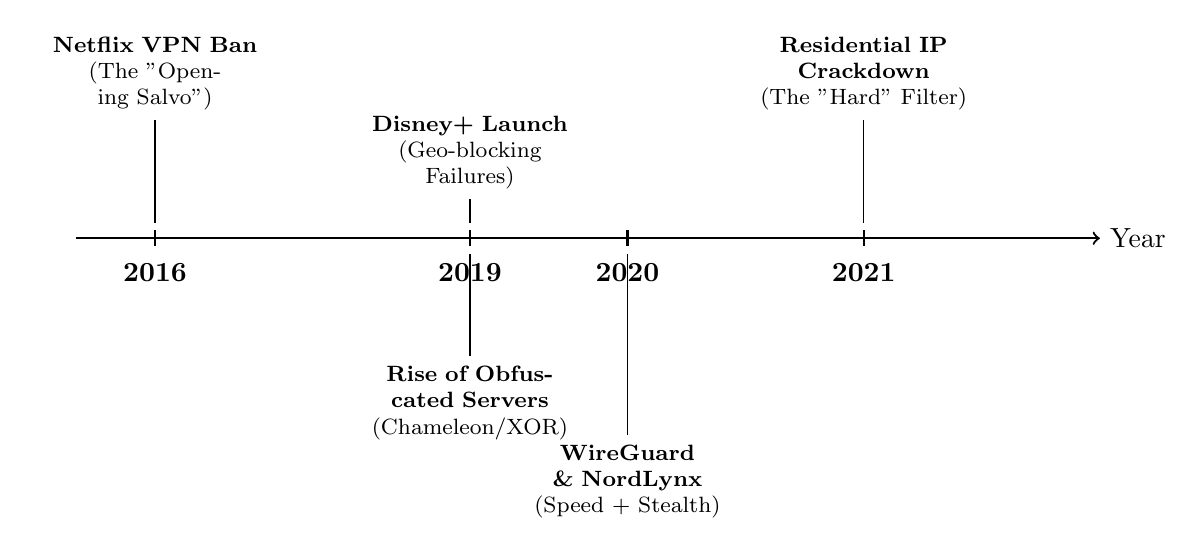
\begin{tikzpicture}[x=2cm, y=1cm]
        % Draw the timeline line
        \draw[->, thick] (0,0) -- (6.5,0) node[right] {Year};
        
        % Ticks and Labels
        \foreach \x/\year in {0.5/2016, 2.5/2019, 3.5/2020, 5.0/2021} {
            \draw[thick] (\x,0.1) -- (\x,-0.1);
            \node[below=0.2cm] at (\x,0) {\textbf{\year}};
        }

        % Events Top (Corporate/Coercive)
        \node[align=center, text width=3cm, above=1.5cm, font=\footnotesize] (netflix16) at (0.5,0) {\textbf{Netflix VPN Ban}\\(The "Opening Salvo")};
        \draw[thin] (0.5,0.2) -- (netflix16);

        \node[align=center, text width=3cm, above=0.5cm, font=\footnotesize] (disney19) at (2.5,0) {\textbf{Disney+ Launch}\\(Geo-blocking Failures)};
        \draw[thin] (2.5,0.2) -- (disney19);
        
        \node[align=center, text width=3cm, above=1.5cm, font=\footnotesize] (resip) at (5.0,0) {\textbf{Residential IP Crackdown}\\(The "Hard" Filter)};
        \draw[thin] (5.0,0.2) -- (resip);

        % Events Bottom (VPN/Adaptive)
        \node[align=center, text width=3cm, below=1.5cm, font=\footnotesize] (obfus) at (2.5,0) {\textbf{Rise of Obfuscated Servers}\\(Chameleon/XOR)};
        \draw[thin] (2.5,-0.2) -- (obfus);

        \node[align=center, text width=3cm, below=2.5cm, font=\footnotesize] (wireguard) at (3.5,0) {\textbf{WireGuard \& NordLynx}\\(Speed + Stealth)};
        \draw[thin] (3.5,-0.2) -- (wireguard);

    \end{tikzpicture}
    \caption{The "Cat-and-Mouse" Timeline: Coercive Barriers vs. Technical Circumvention.}
    \label{fig:timeline}
\end{figure}

This timeline illustrates that corporate enforcement often lags behind consumer innovation. The 2016 ban forced VPNs to adopt "Obfuscated Servers" (2019), which in turn prompted Netflix to block "Residential IPs" (2021).

\section{Limitations and Validity}
While this study provides a novel quantitative framework for analyzing geo-arbitrage, several limitations must be acknowledged to contextualize the findings.

\subsection{Sample Size and Generalizability}
The correlation analysis relies on a strategic sample of $N=11$ major digital service providers. While these firms represent a significant majority of the consumer subscription market by capitalization, the sample is small in statistical terms. Consequently, the findings should be interpreted as "exploratory" evidence of strategic archetypes rather than a definitive "law" of digital economics. Future research could expand this dataset to include mid-tier SaaS providers to test if the "Enterprise Fortress" model holds for smaller B2B firms.

\subsection{The "Average Citizen" Bias (Socioeconomic Mismatch)}
Our "Affordability" metric calculates cost as a percentage of the \textit{Average National Monthly Wage}. However, in emerging markets like Turkey or Argentina, the target demographic for services like Netflix or Adobe is likely the urban upper-middle class, whose income is significantly higher than the national average. 

For instance, World Bank data and local surveys indicate that in Turkey, the top 20\% of earners capture nearly 48\% of the total disposable income. Similarly, in Argentina, the top 10\% of earners have an average monthly income exceeding \$496 USD, well above the national median. This implies that global digital services are aggressively priced to target this specific "Global Elite" segment. As \textcite{kastanakis2012between} argue, in markets with high income inequality, luxury consumption (and by extension, premium digital subscriptions) serves as a critical status signal for the upper class. Use of this "Elite" pricing strategy explains why firms tolerate some level of piracy from the lower 80\%—they were never the customers to begin with.

\subsection{Temporal Sensitivity in Volatile Markets}
The Digital Services Price Index (DSPI) represents a snapshot of pricing data from late 2024. In hyper-inflationary economies such as Argentina and Turkey, local currency prices are adjusted frequently. A "Cheap" arbitrage opportunity identified in this thesis could be eroded effectively overnight by a price hike or currency devaluation. The "Arbitrage Window" is therefore dynamic, not static.

\subsection{AI Classification Reliability}
The use of Large Language Models (Gemini 3 Flash) introduces a potential "Black Box" validity risk. To mitigate this, we utilized the model's self-reported confidence scores as a filtering mechanism. The final dataset achieved an average confidence score of \textbf{0.947}, with \textbf{80.5\%} of classifications exceeding a confidence threshold of 0.9. This high degree of certainty suggests that the detection of "coercive" vs. "general" language is robust, even without human-in-the-loop verification for every datapoint.
